\section{Presentation Logic Layer}

%What pages will be present in your project? briefly indicate how your website will be organized

\hspace{5mm}DamacaNaN will have a welcome, login, register, homepage, about us, search, profile, posts, post view, add post, edit post, message, pages. When users are logged or registered, they will be directed to the home page. Otherwise, they will be stuck on the login/register page and cannot get on the website. After the login/register operation, they can surf through other pages indicated above. \newline


We have designed 9 mockup pages. They are welcome, register, login, profile, main page, post view, post addition, post edition, message page you can see then at below 
\subsection{Mockup Pages:}

%For the main pages put a mockup and describe it in detail.

\begin{center}
    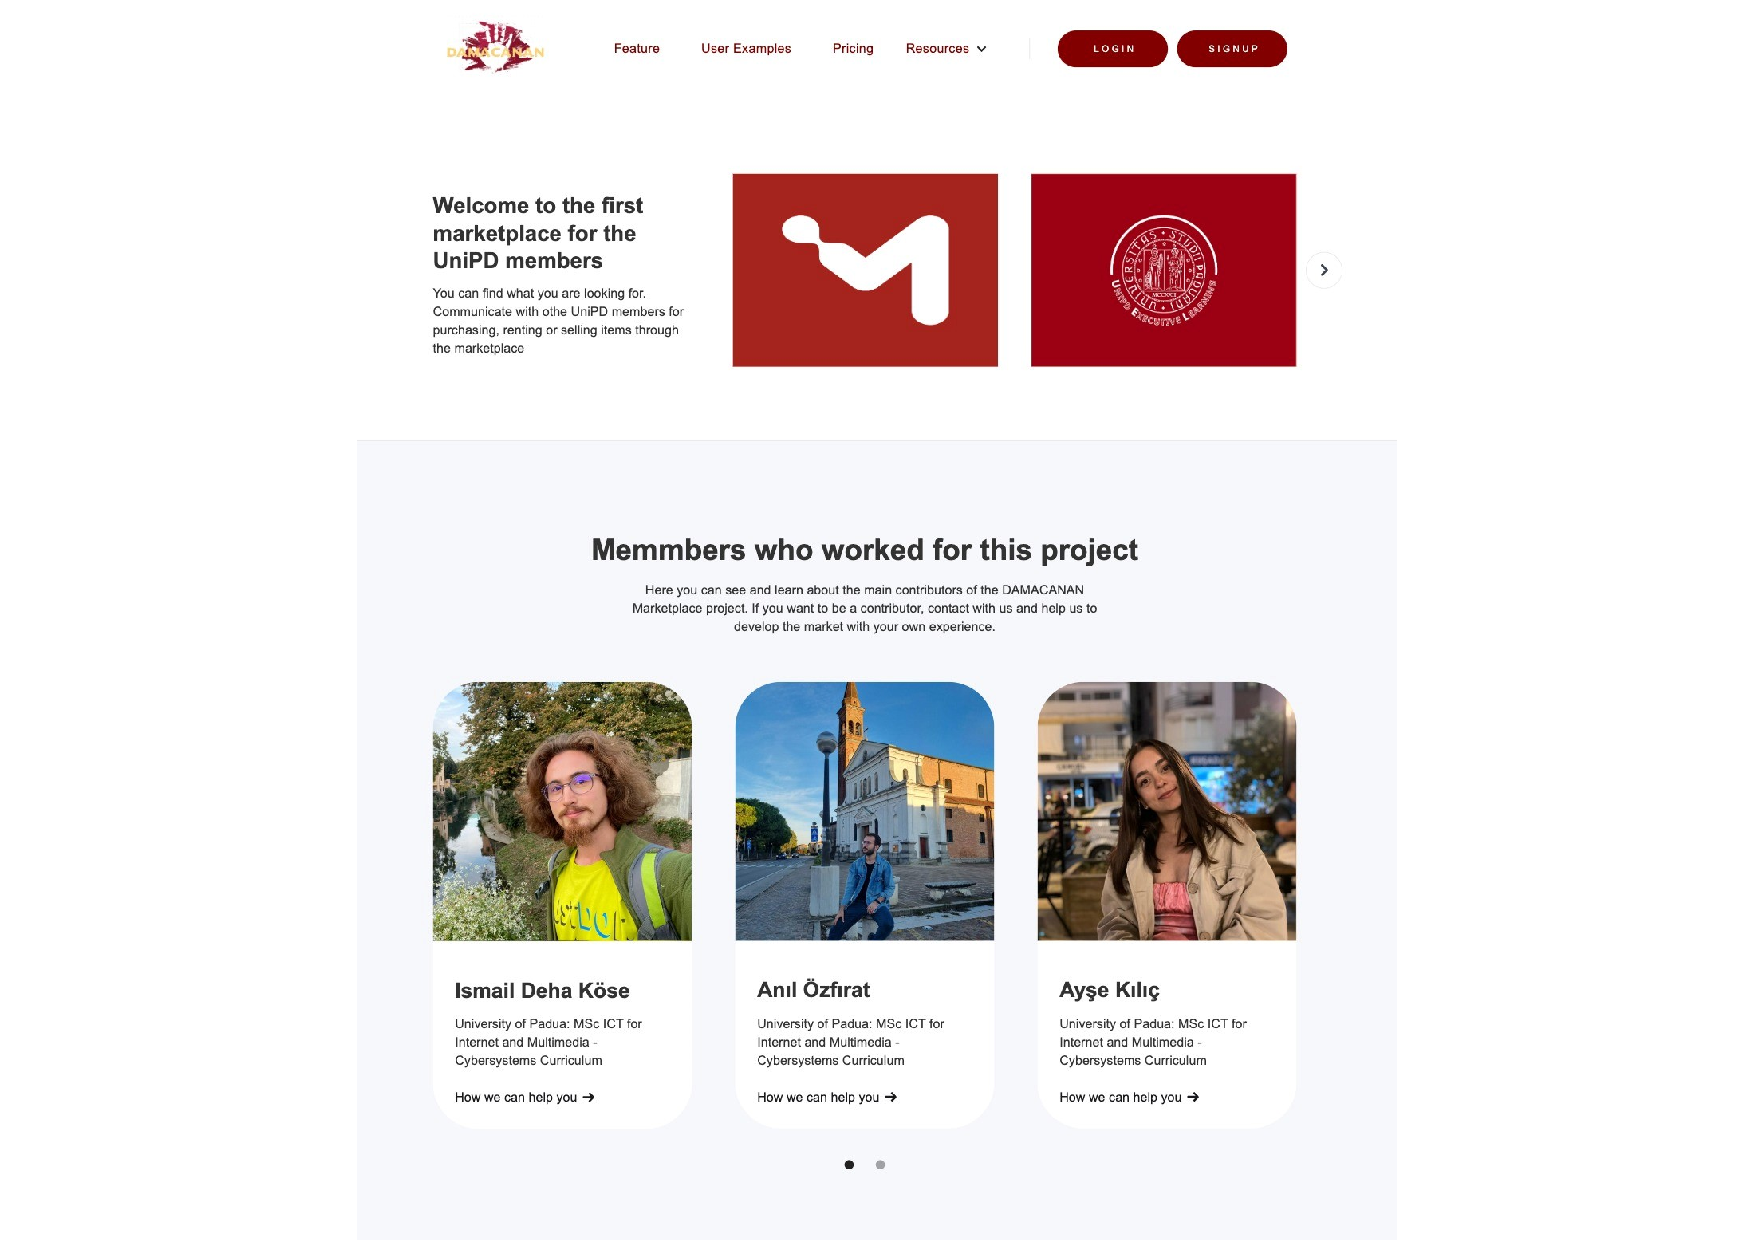
\includegraphics[scale = 0.7, center]{Mockup/mockup.pdf}
\caption{Home Page Mockup}
\label{fig:my_label}



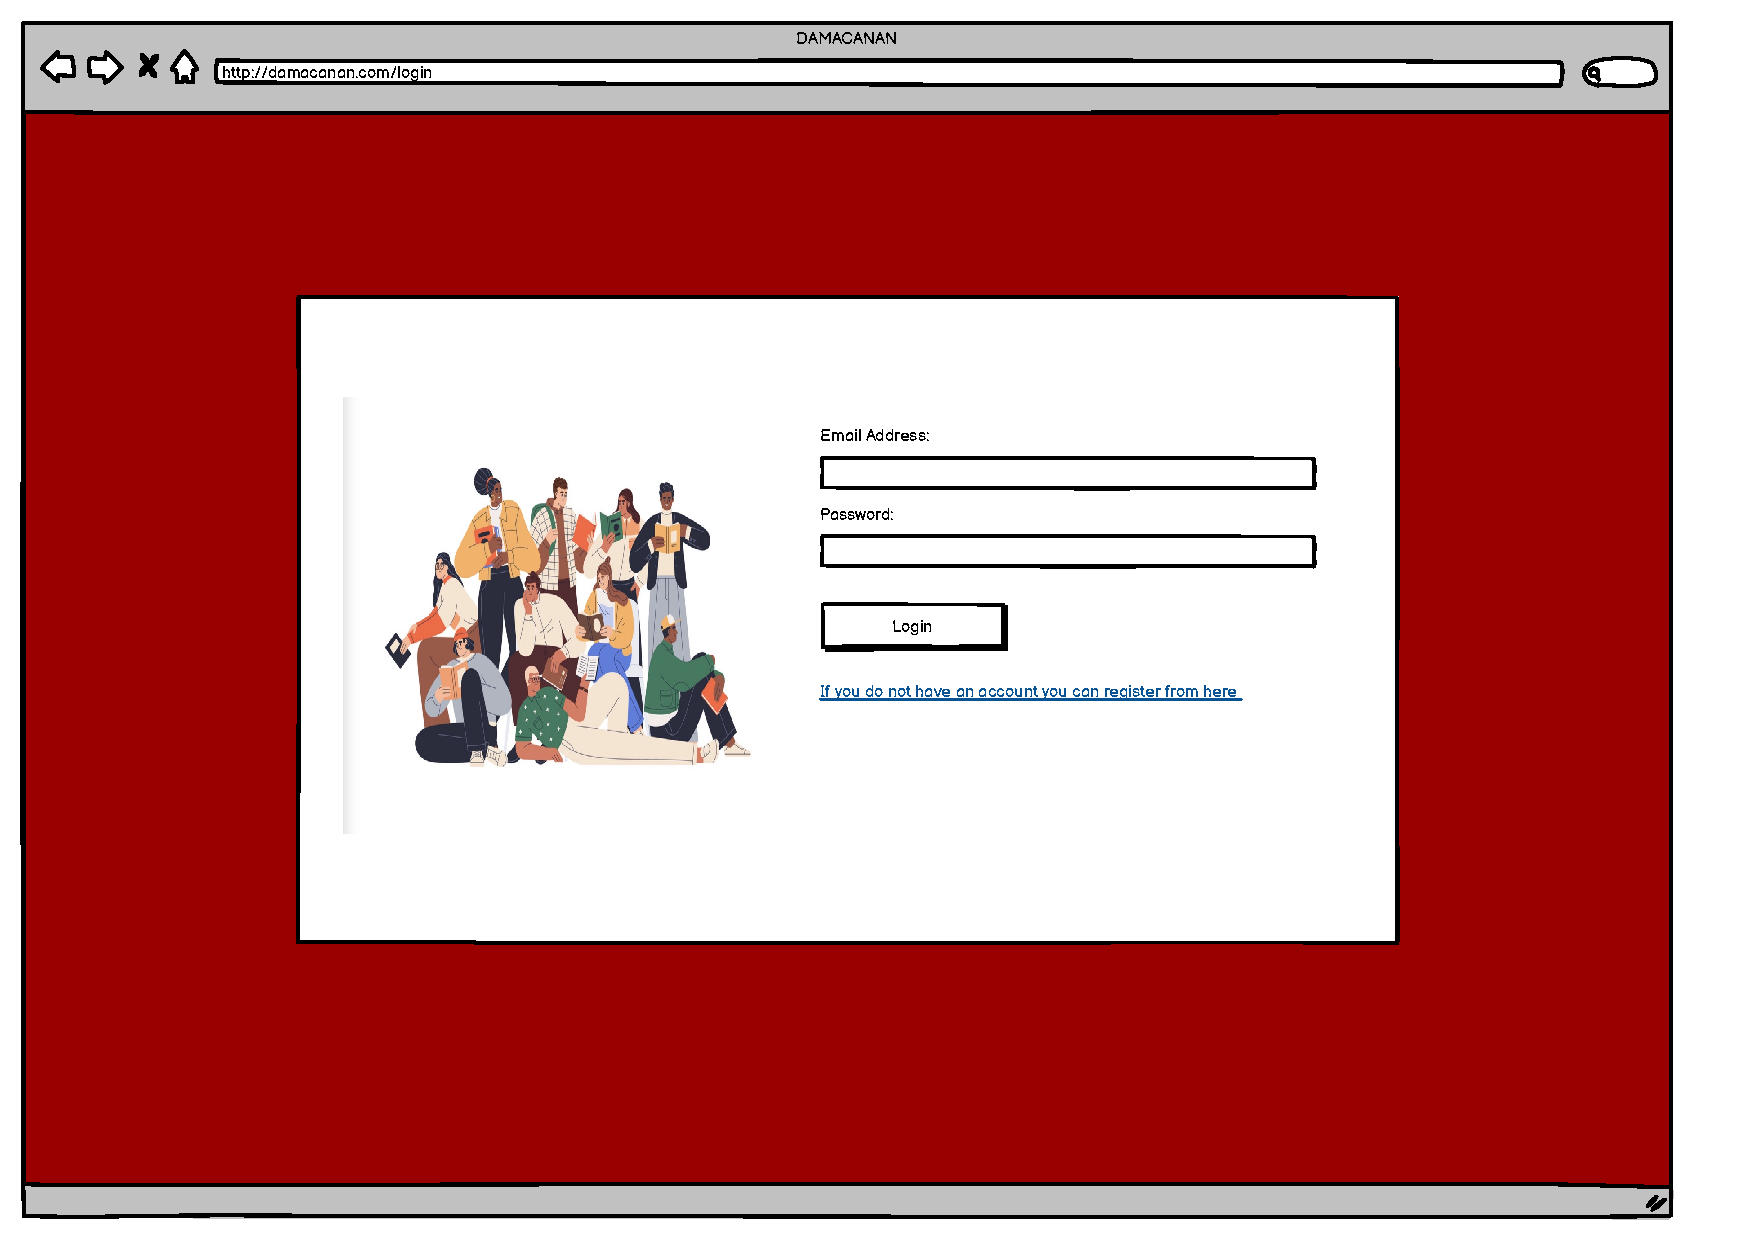
\includegraphics[scale = 0.7, center]{Mockup/Login_Page_Mockup.pdf}
\caption{Login Page Mockup}
\label{fig:my_label}




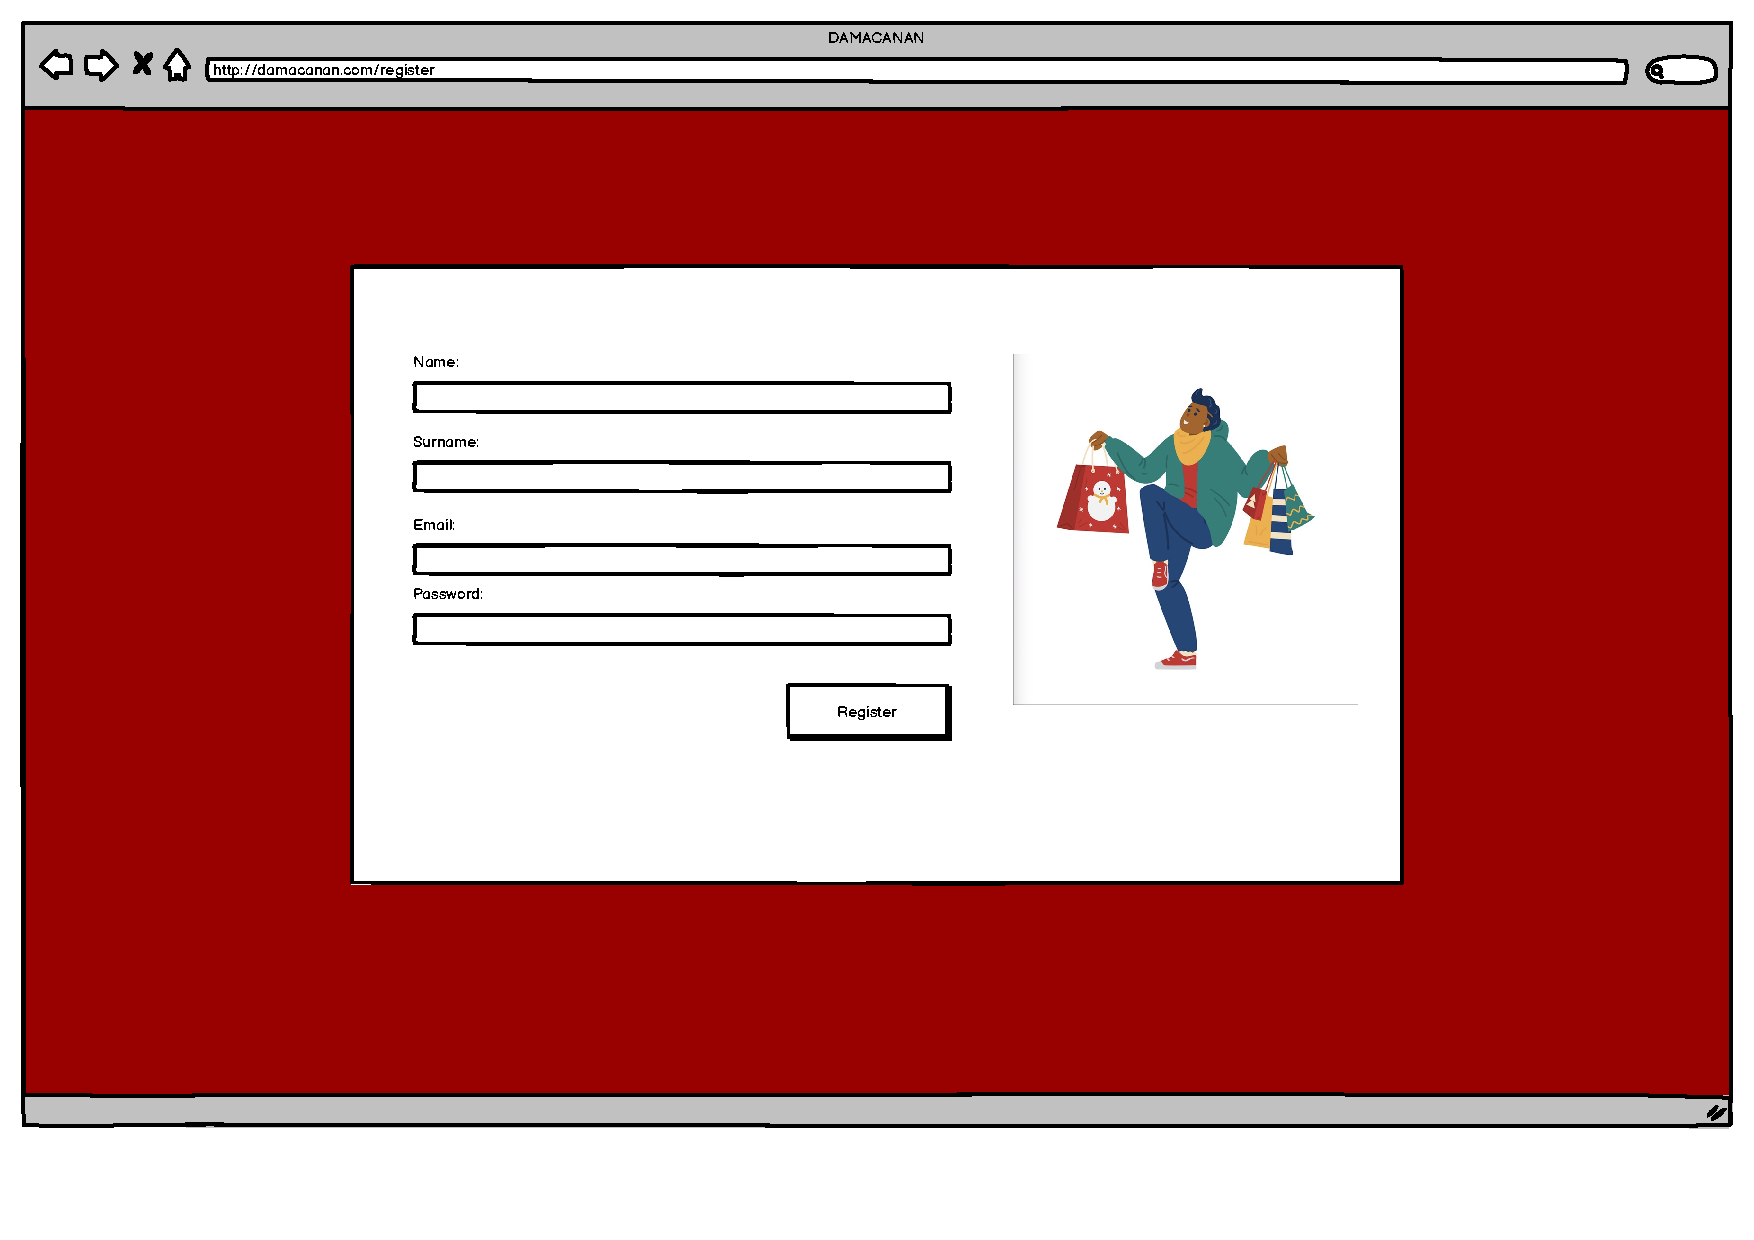
\includegraphics[scale = 0.7, center]{Mockup/Register_Page_Mockup.pdf}
\caption{Register Page Mockup}
\label{fig:my_label}




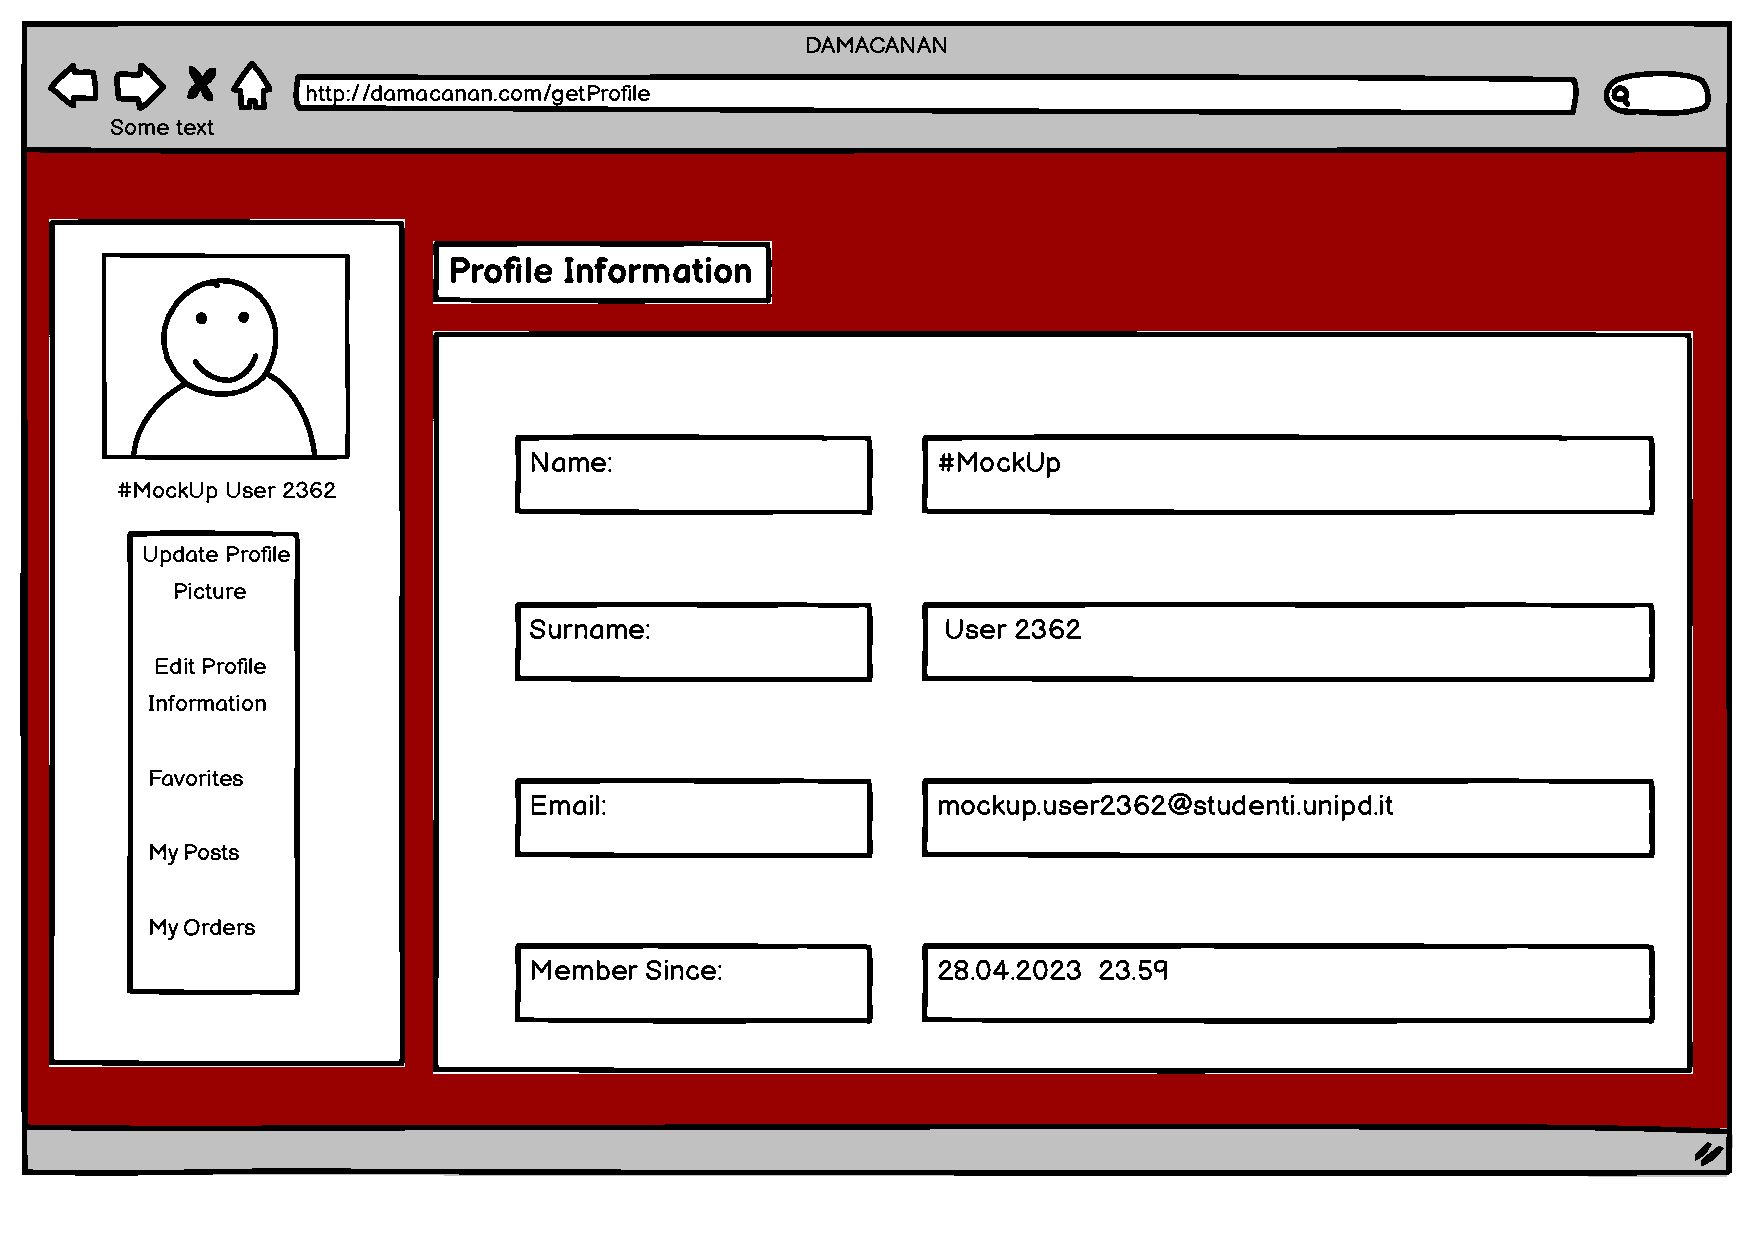
\includegraphics[scale = 0.7, center]{Mockup/Profile_Page_Mockup.pdf}
\caption{Profile Page Mockup}
\label{fig:my_label}




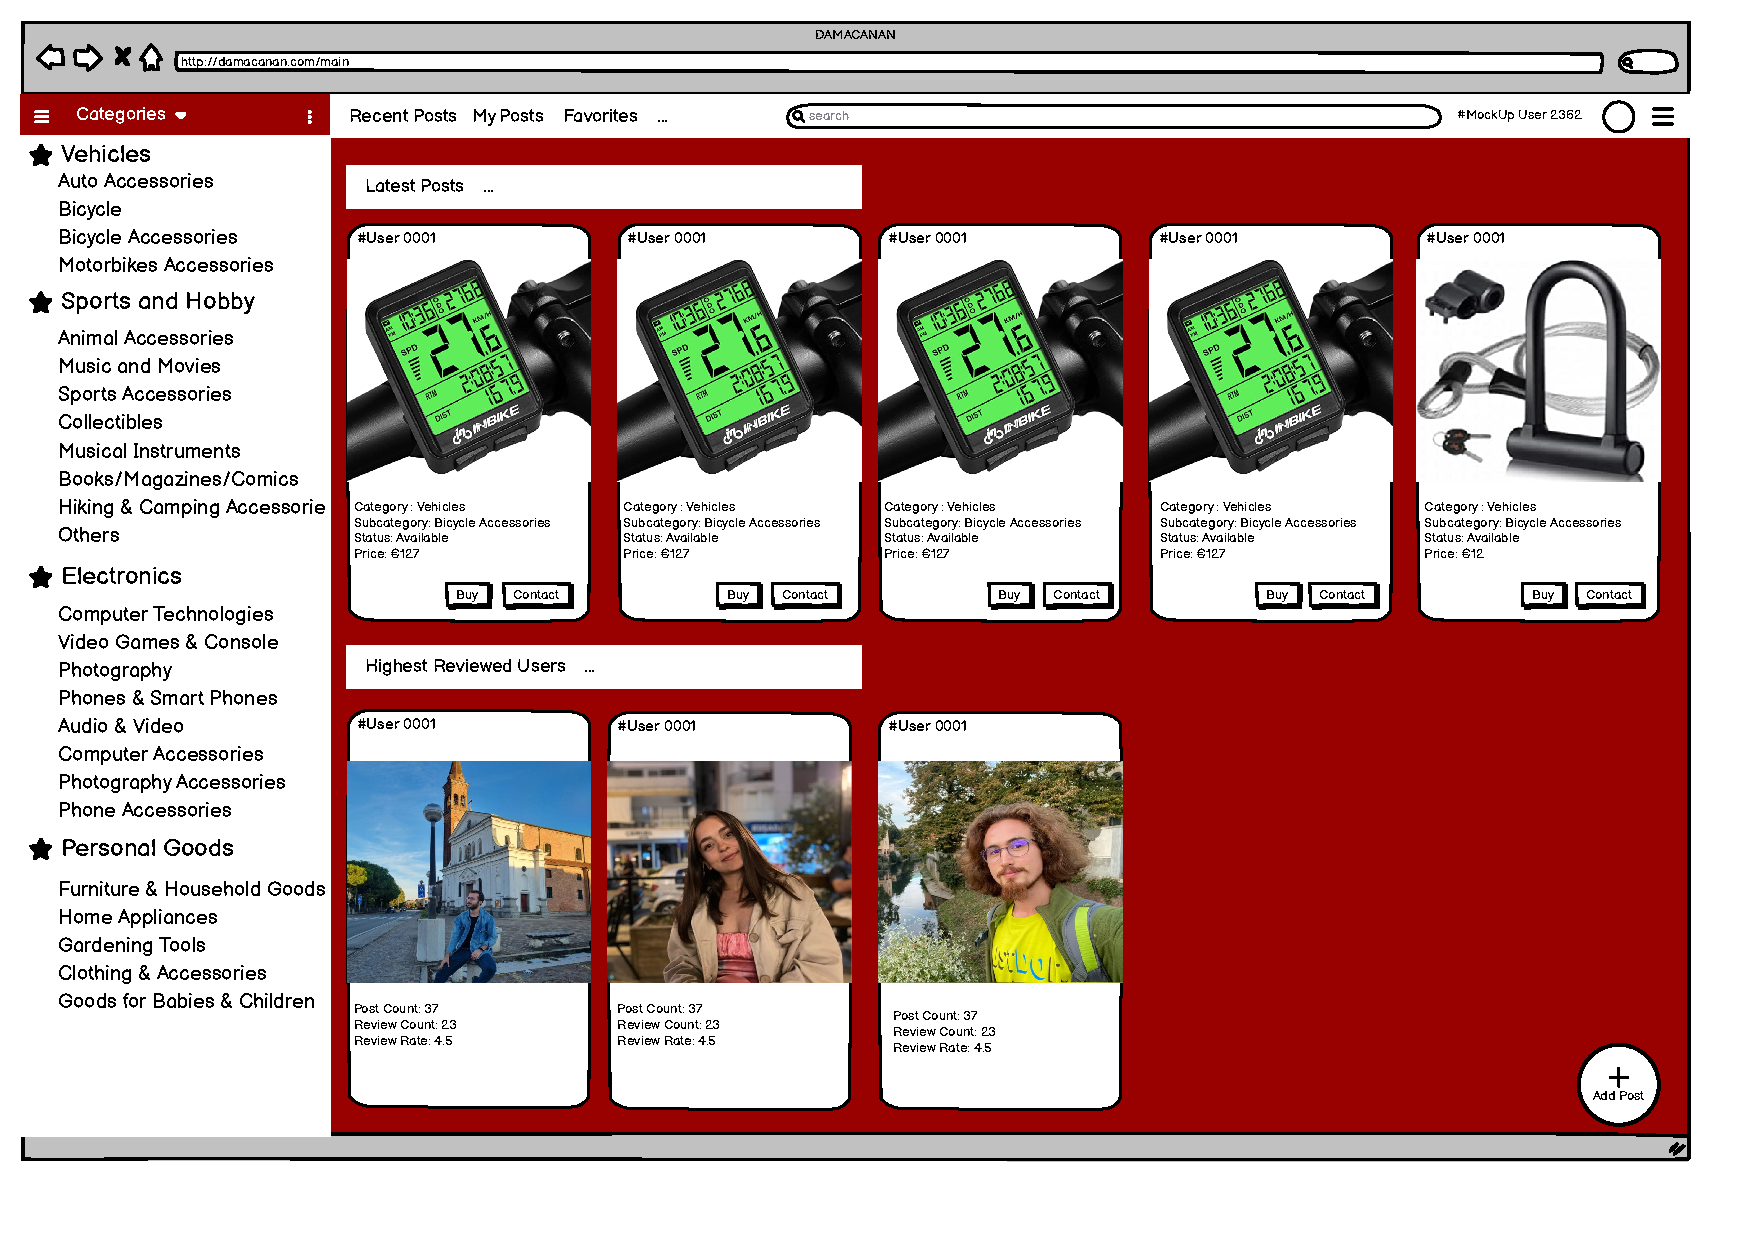
\includegraphics[scale = 0.7, center]{Mockup/Main_Page_Mockup.pdf}
\caption{Home Page Mockup}
\label{fig:my_label}




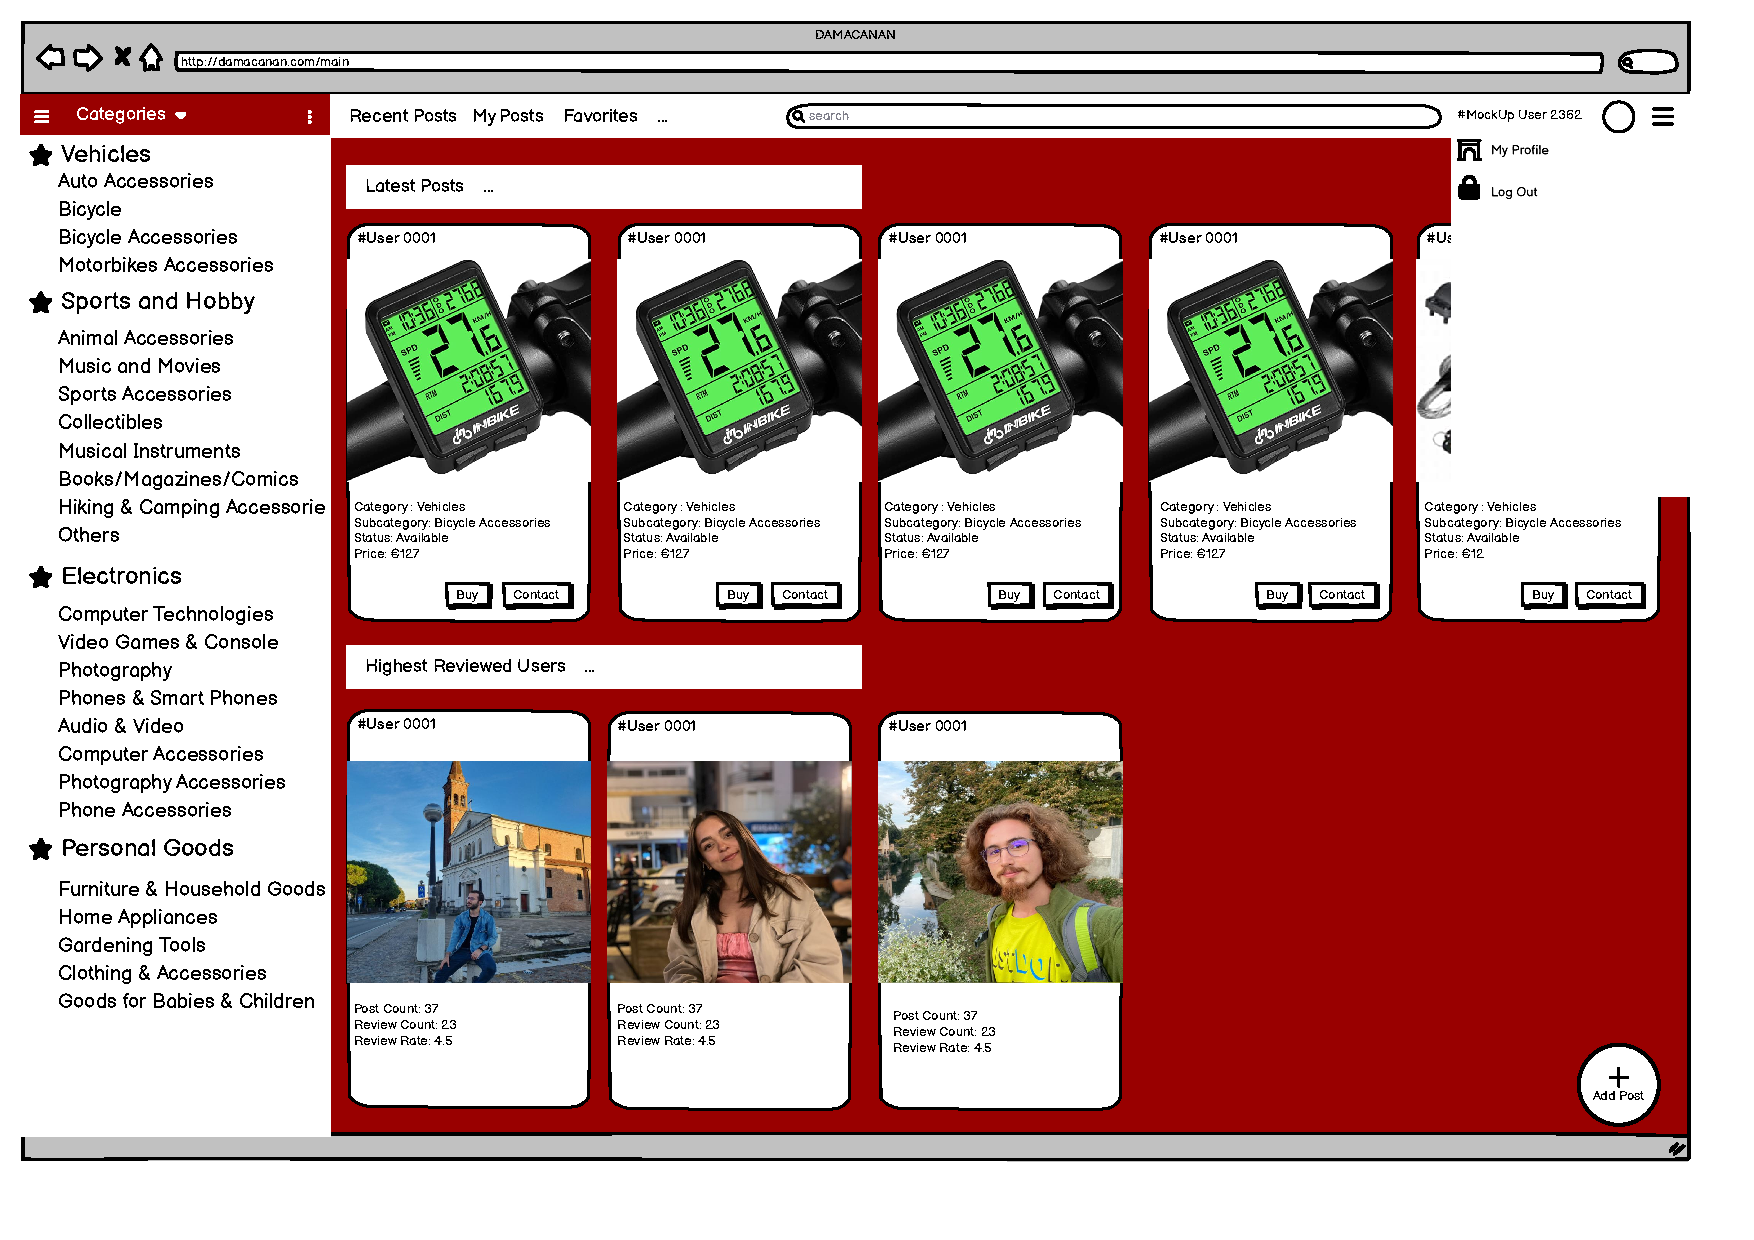
\includegraphics[scale = 0.7, center]{Mockup/Main_Page_ProfieBar_Mockup.pdf}
\caption{Home Page Profile Bar Mockup}
\label{fig:my_label}




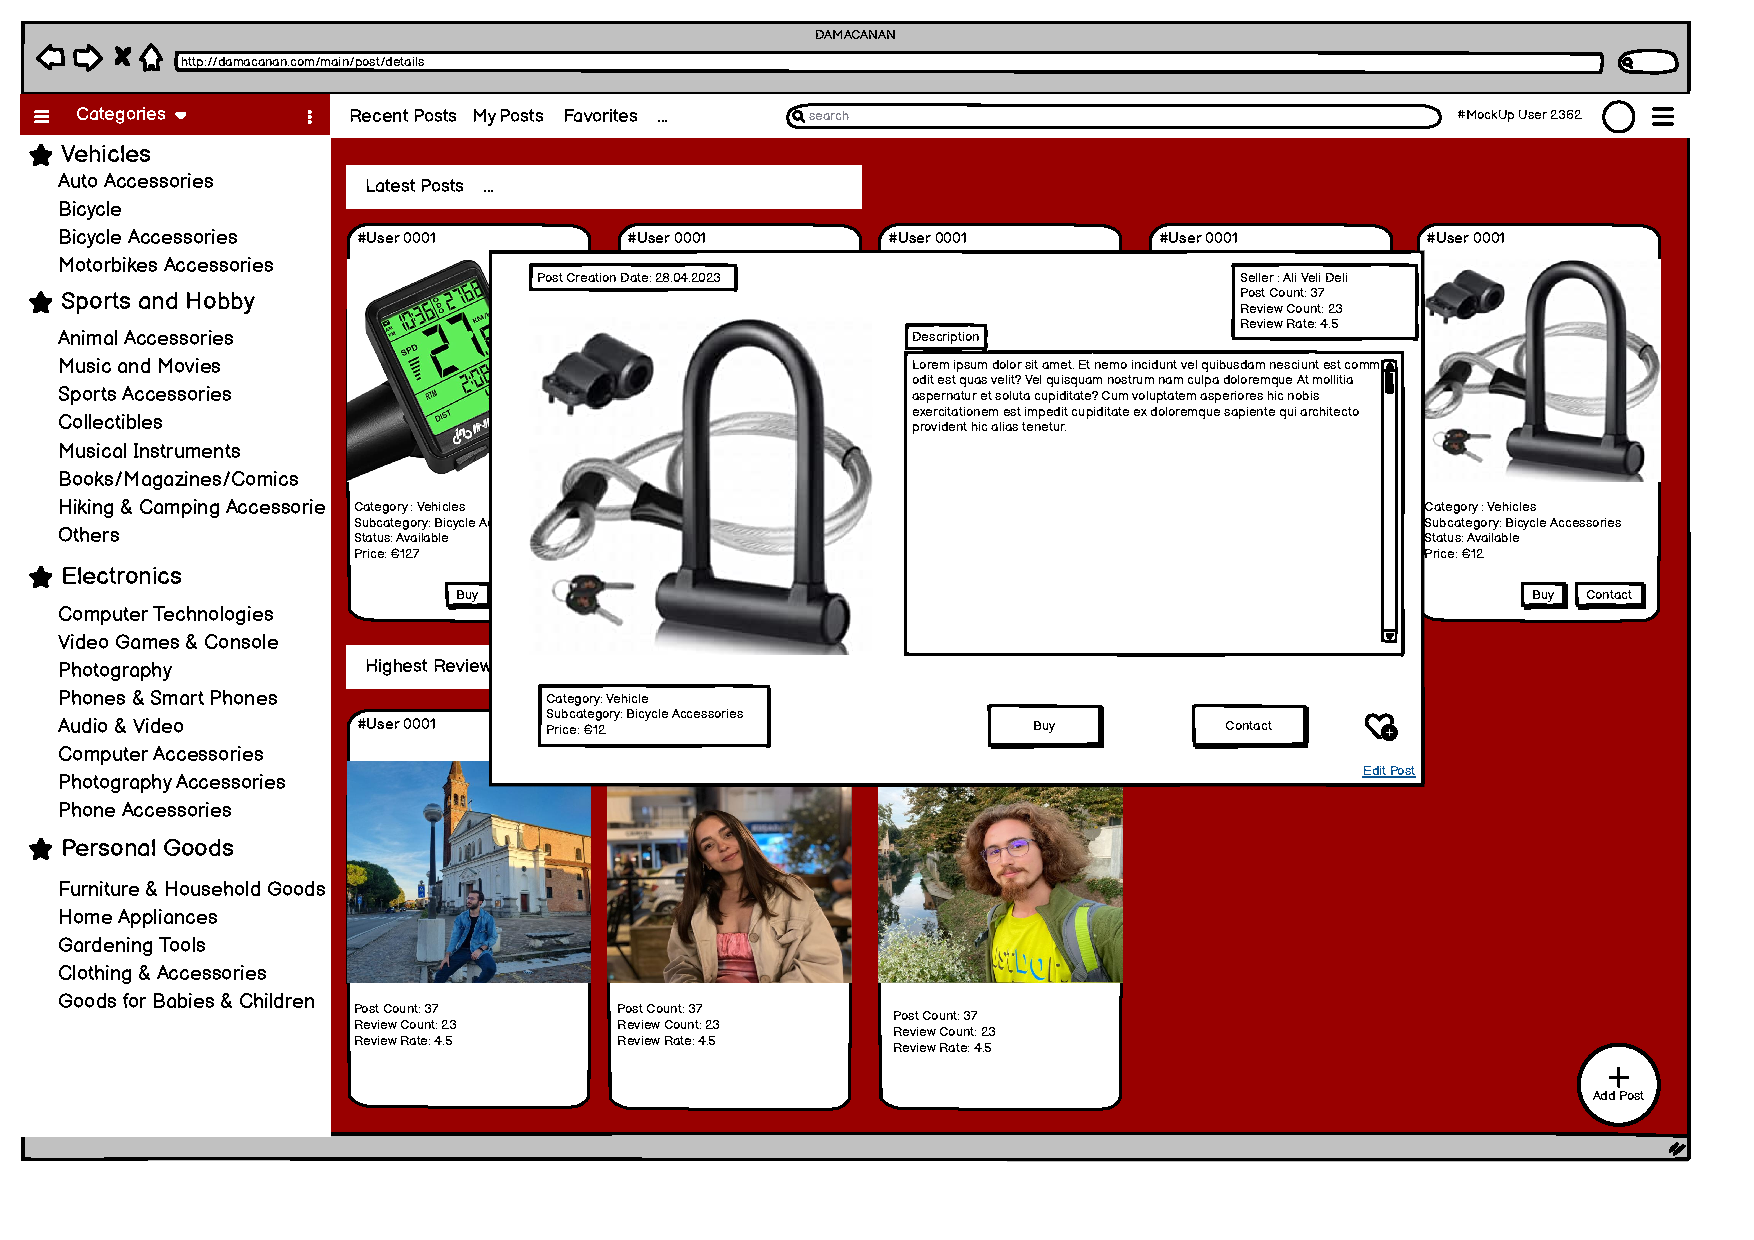
\includegraphics[scale = 0.7, center]{Mockup/Post_View_Mockup.pdf}
\caption{Post View Page Mockup}
\label{fig:my_label}



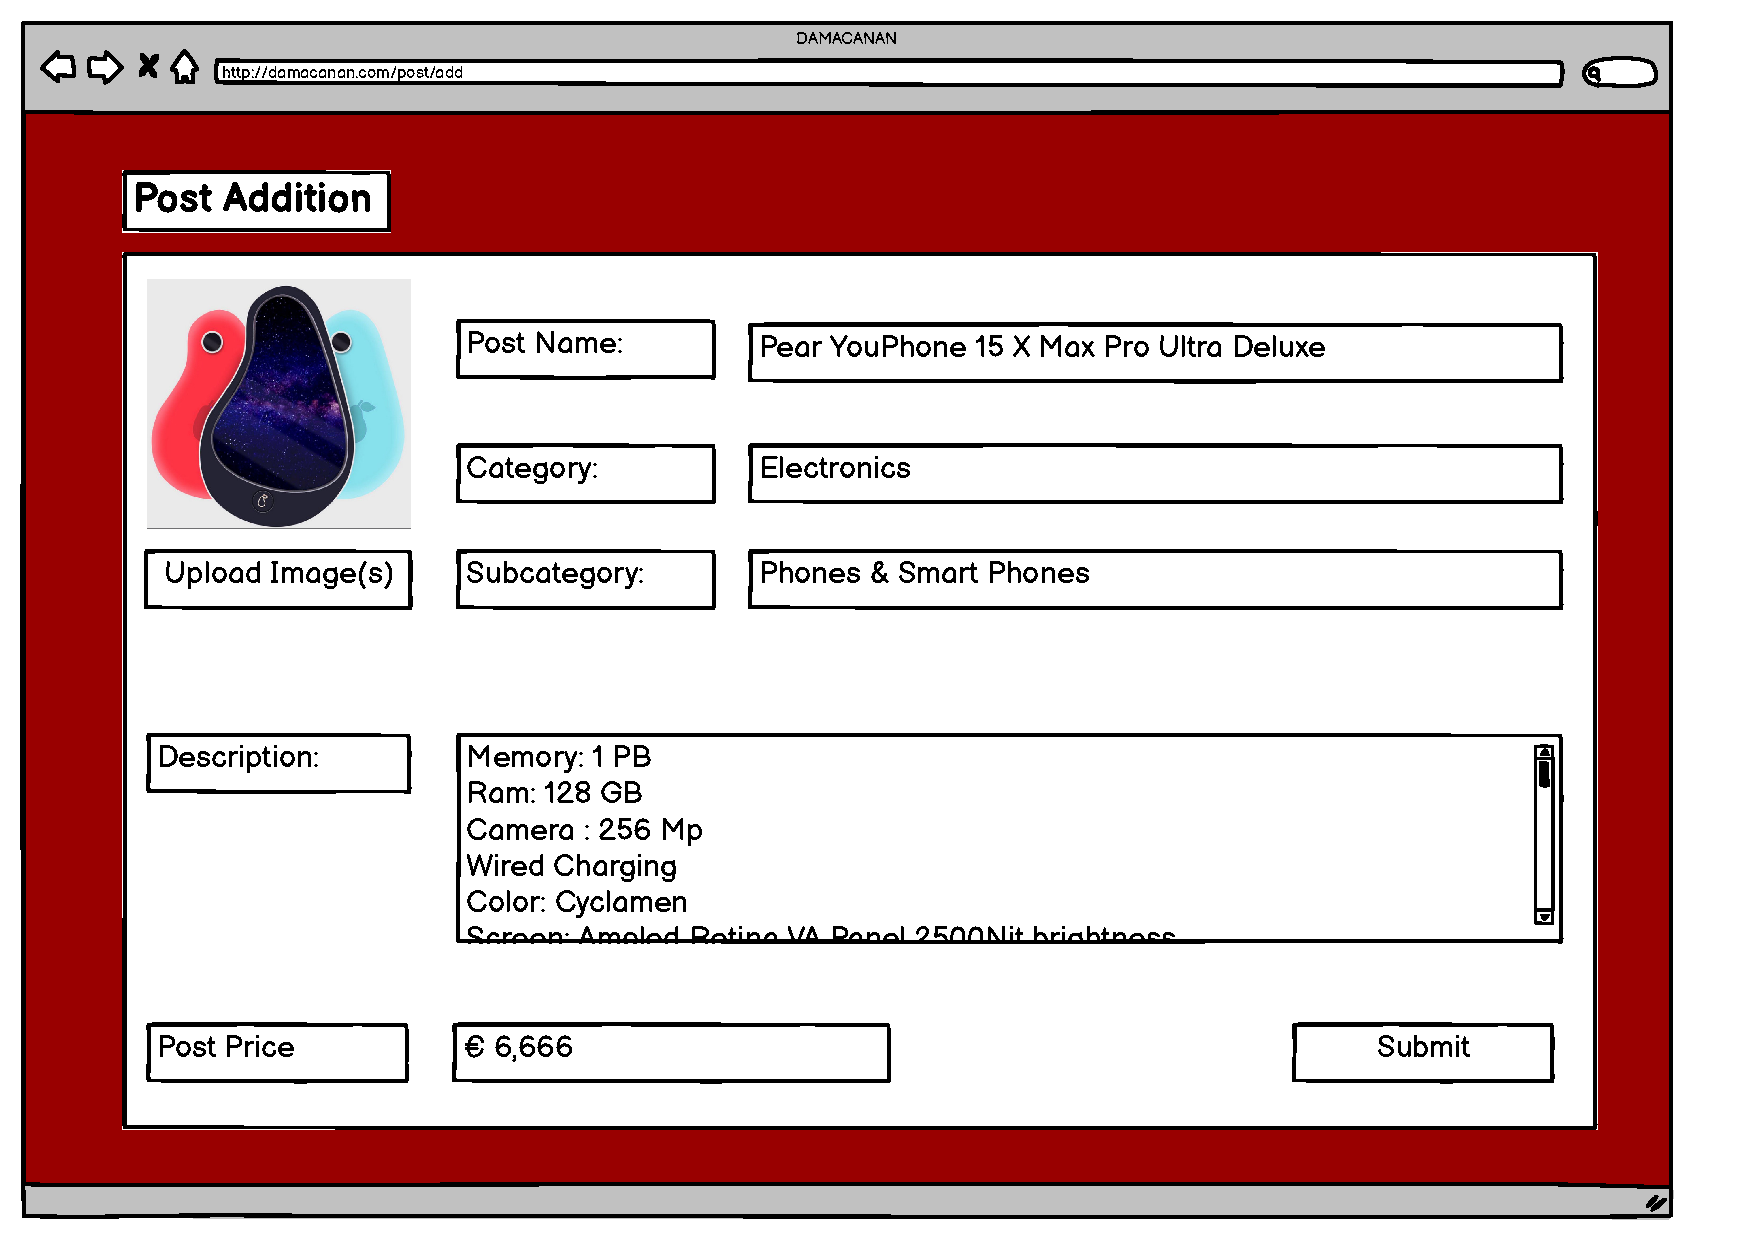
\includegraphics[scale = 0.7, center]{Mockup/Post_Add_Mockup.pdf}
\caption{Post Addition Page Mockup}
\label{fig:my_label}




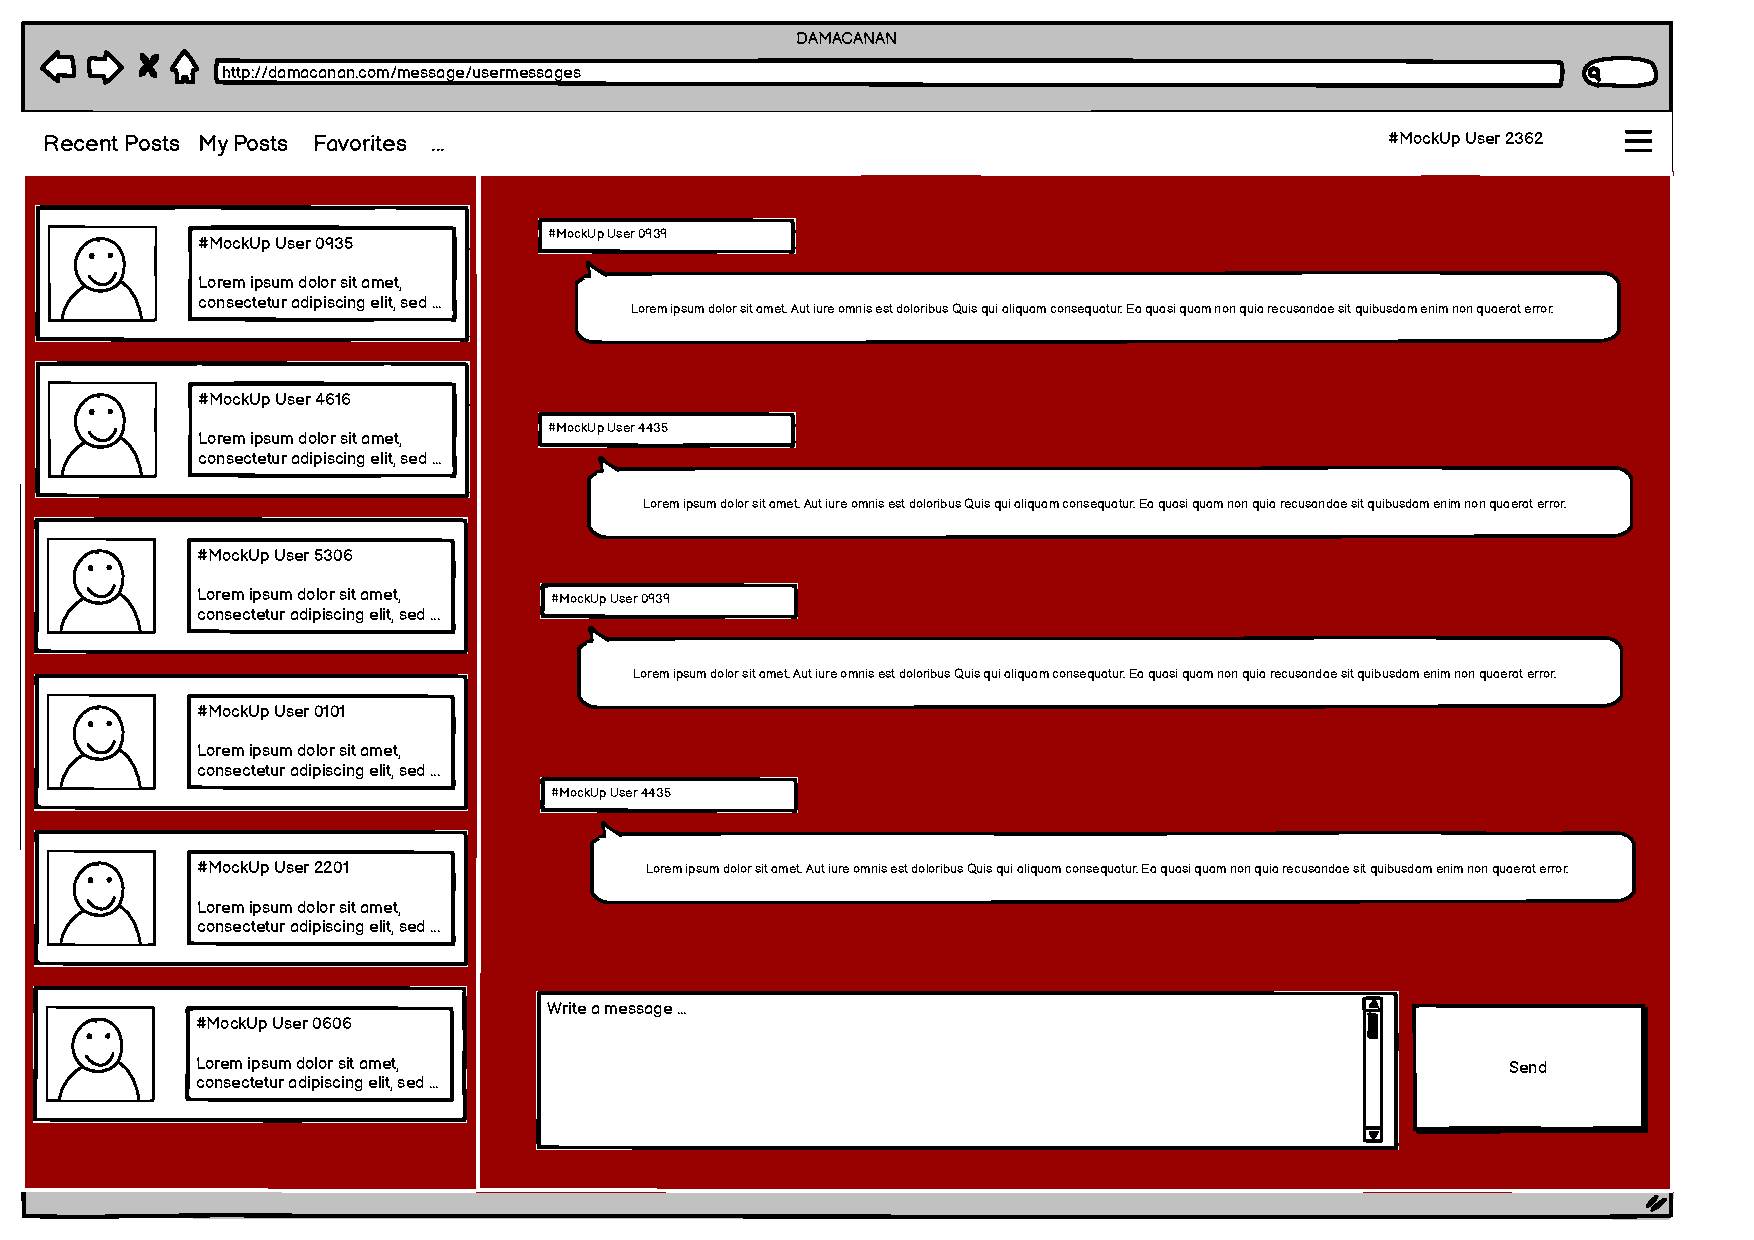
\includegraphics[scale = 0.7, center]{Mockup/Message_Page_Mockup.pdf}
\caption{Message Page Mockup}
\label{fig:my_label}




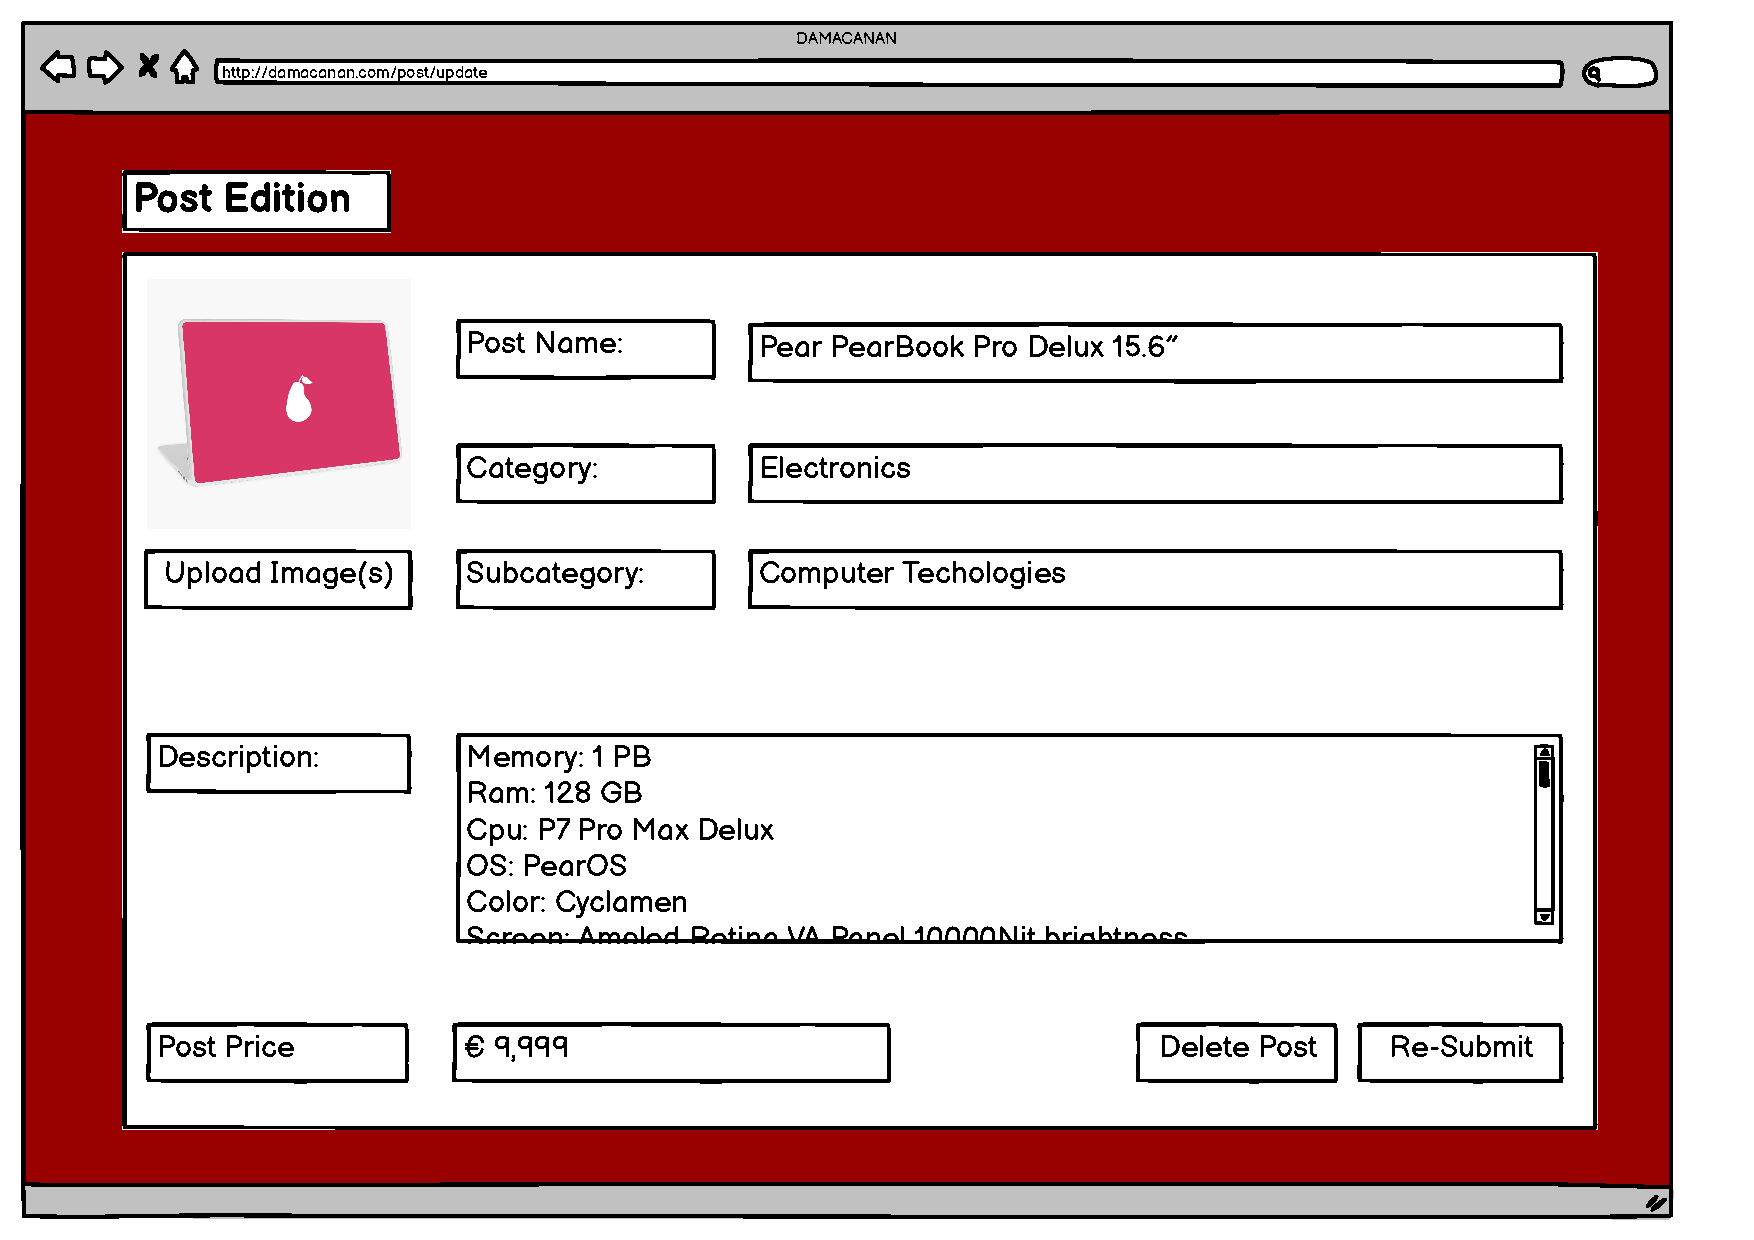
\includegraphics[scale = 0.7, center]{Mockup/Post_Edit_Mockup.pdf}
\caption{Post Edition Page Mockup}
\label{fig:my_label}
\end{center} \newline




\textbf{Welcome Page},  there is a short introduction about our website, and at the bottom, you can see the creators of the "DamacaNaN" website. At the top of the website, you can see some buttons to click. At the top right corner, you can see the login and register buttons. \newline

\textbf{The Sign in and log-in pages,} both of them, are like traditional register and login pages. \newline

\textbf{The profile page,} is an editable page for just profile owners, others just see the information such as profile picture (if exists), name, surname, email and date of their membership. Password specifically can be seen and edited just by the owner of the account. \newline

\textbf{Home Page, }this page is only visible after the login operation, so if and only if registered users can see this page. This page has posts that lasted added, users who have the highest review point, a search bar that can search what you want, a category bar that has categories, and next to the below of categories themselves subcategories. Also, this page has a profile bar that can visit the profile and get logged out. \newline

\textbf{Post view page}, when get into the post in which you are interested, there will be post pictures (bigger than the previous page), post descriptions, seller part which has some seller information such as a profile picture (if exists), name, and surname, post count, review count, review rate (if exists). \newline

\textbf{Post addition page,} sellers can create their posts here. They can add pictures, descriptions, categories, subcategories, and prices about the post.\newline

\textbf{Post edition page,} sellers can update or change their posts here. They can update or change pictures, descriptions, categories, subcategories, and prices about the post. In addition, you can delete your post.\newline

